% Options for packages loaded elsewhere
\PassOptionsToPackage{unicode}{hyperref}
\PassOptionsToPackage{hyphens}{url}
%
\documentclass[
]{article}
\author{}
\date{\vspace{-2.5em}}

\usepackage{amsmath,amssymb}
\usepackage{lmodern}
\usepackage{iftex}
\ifPDFTeX
  \usepackage[T1]{fontenc}
  \usepackage[utf8]{inputenc}
  \usepackage{textcomp} % provide euro and other symbols
\else % if luatex or xetex
  \usepackage{unicode-math}
  \defaultfontfeatures{Scale=MatchLowercase}
  \defaultfontfeatures[\rmfamily]{Ligatures=TeX,Scale=1}
\fi
% Use upquote if available, for straight quotes in verbatim environments
\IfFileExists{upquote.sty}{\usepackage{upquote}}{}
\IfFileExists{microtype.sty}{% use microtype if available
  \usepackage[]{microtype}
  \UseMicrotypeSet[protrusion]{basicmath} % disable protrusion for tt fonts
}{}
\makeatletter
\@ifundefined{KOMAClassName}{% if non-KOMA class
  \IfFileExists{parskip.sty}{%
    \usepackage{parskip}
  }{% else
    \setlength{\parindent}{0pt}
    \setlength{\parskip}{6pt plus 2pt minus 1pt}}
}{% if KOMA class
  \KOMAoptions{parskip=half}}
\makeatother
\usepackage{xcolor}
\IfFileExists{xurl.sty}{\usepackage{xurl}}{} % add URL line breaks if available
\IfFileExists{bookmark.sty}{\usepackage{bookmark}}{\usepackage{hyperref}}
\hypersetup{
  hidelinks,
  pdfcreator={LaTeX via pandoc}}
\urlstyle{same} % disable monospaced font for URLs
\usepackage[margin=1in]{geometry}
\usepackage{graphicx}
\makeatletter
\def\maxwidth{\ifdim\Gin@nat@width>\linewidth\linewidth\else\Gin@nat@width\fi}
\def\maxheight{\ifdim\Gin@nat@height>\textheight\textheight\else\Gin@nat@height\fi}
\makeatother
% Scale images if necessary, so that they will not overflow the page
% margins by default, and it is still possible to overwrite the defaults
% using explicit options in \includegraphics[width, height, ...]{}
\setkeys{Gin}{width=\maxwidth,height=\maxheight,keepaspectratio}
% Set default figure placement to htbp
\makeatletter
\def\fps@figure{htbp}
\makeatother
\setlength{\emergencystretch}{3em} % prevent overfull lines
\providecommand{\tightlist}{%
  \setlength{\itemsep}{0pt}\setlength{\parskip}{0pt}}
\setcounter{secnumdepth}{-\maxdimen} % remove section numbering
\usepackage{float}
\usepackage{sectsty}
\usepackage{caption}
\captionsetup[figure]{labelformat=empty}
\ifLuaTeX
  \usepackage{selnolig}  % disable illegal ligatures
\fi

\begin{document}

\bibliographystyle{apalike-fr}

\hypertarget{annexes}{%
\section{Annexes}\label{annexes}}

\hypertarget{annexes-du-chapitre-3}{%
\subsection{Annexes du Chapitre 3}\label{annexes-du-chapitre-3}}

\hypertarget{appendix-1-the-mathematical-development-of-the-bmf-test-bmw-test-and-bmf-test-numerical-example}{%
\subsubsection{\texorpdfstring{Appendix 1 : The Mathematical Development
of the \(\bm{F}\)-test, \(\bm{W}\)-test, and \(\bm{F^*}\)-test:
Numerical
Example}{Appendix 1 : The Mathematical Development of the \textbackslash bm\{F\}-test, \textbackslash bm\{W\}-test, and \textbackslash bm\{F\^{}*\}-test: Numerical Example}}\label{appendix-1-the-mathematical-development-of-the-bmf-test-bmw-test-and-bmf-test-numerical-example}}

Descriptive statistics are presented in Table A1. The raw data are
available here :
\url{https://github.com/mdelacre/W-ANOVA/tree/master/Functions} (see
``practical example.R''). The dependent variable is a score that can
vary from 0 to 40. The independent variable is a three-level factor A
(levels = \(A_1\), \(A_2\) and \(A_3\)).

\begin{figure}
\includegraphics[width=1\linewidth]{C:/Users/mdelacre/Documents/Github project/W-ANOVA/Rmarkdown folder/Rmarkdown inputs/TableA1} \end{figure}

The overall mean (i.e.~the mean of the global dataset) is a weighted
mean of the sample means :

\[\bar{X_{..}}=\frac{(41\times24)+(21\times23)+(31\times27)}{41+21+31}=\frac{2304}{93} \approx 24.77\]
The \emph{F}-test statistic and degrees of freedom are computed by
applying equation (1) and related degrees of freedom :

\[
F=\frac{\frac{1}{3-1}[41\times(24-\frac{2304}{93})^2+21\times(23-\frac{2304}{93})^2+31\times(27-\frac{2304}{93})^2]}
{\frac{1}{93-3}[(41-1)\times81.75+(21-1)\times10.075+(31-1)\times38.4]} \approx 2.377
\]

\[
df_n=3-1=2
\]

\[
df_d=93-3=90
\] The \(F^*\)-test statistic and his degrees of freedom are computed by
applying equation (2) and related degrees of freedom :

\[
F^*=\frac{41\times(24-\frac{2304}{93})^2+21\times(23-\frac{2304}{93})^2+31\times(27-\frac{2304}{93})^2}{(1-\frac{41}{93})\times81.75+(1-\frac{21}{93})\times10.075+(1-\frac{31}{93})\times38.4} \approx 3.088
\]

\[
df_n=3-1=2
\]

\[
df_d=\frac{1}{\frac{(\frac{(1-\frac{41}{93})\times81.75}{\sum_{j=1}^k(1-\frac{n_j}{N})S_j^2})^2}{41-1}+\frac{(\frac{(1-\frac{21}{93})\times10.075}{\sum_{j=1}^k(1-\frac{n_j}{N})S_j^2})^2}{21-1}+\frac{(\frac{(1-\frac{31}{93})\times38.4}{\sum_{j=1}^k(1-\frac{n_j}{N})S_j^2})^2}{31-1}} \approx 81.149
\]

where \(\sum_{j=1}^k(1-\frac{n_j}{N})\times S_j^2 \approx 79.11\)

Finally, the \emph{W}-test and his degrees of freedom are computed by
applying equation (3) and related degrees of freedom :

\[
W=\frac{\frac{1}{3-1}[\frac{41}{81.75}(24-\bar{X'})^2+\frac{21}{10.075}(23-\bar{X'})^2+\frac{31}{38.4}(27-\bar{X'})^2]}
{\frac{2(3-2)}{3^2-1}[(\frac{1}{41-1})(1-\frac{\frac{41}{81.75}}{w})^2+(\frac{1}{21-1})(1-\frac{\frac{21}{10.075}}{w})^2+(\frac{1}{31-1})(1-\frac{\frac{31}{38.4}}{w})^2]+1} \approx 4.606
\]

where: \(w=\sum_{j=1}^k w_j \approx 3.39\) and
\(\bar{X'}=\frac{\sum_{j=1}^k (w_j\bar{X_j})}{w} \approx 24.1\)

\[
df_n=3-1
\]

\[
df_d=\frac{3^2-1}{3[\frac{(1-\frac{w_j}{w})^2}{41-1}+\frac{(1-\frac{w_j}{w})^2}{21-1}+\frac{(1-\frac{w_j}{w})^2}{31-1}]} \approx 59.32
\]

One should notice that in this example, the biggest sample size has the
biggest variance. As previously mentioned, it means that the
\emph{F}-test will be too conservative, because the \emph{F} value
decreases. The \emph{F}*-test will also be a little too conservative,
even if the test is less affected than the \emph{F}-test. As a
consequence: \(W\) \textgreater{} \(F^*\) \textgreater{} \(F\).

\hypertarget{appendix-2-justification-for-the-choice-of-distributions-in-simulations}{%
\subsubsection{Appendix 2 : Justification for the choice of
distributions in
simulations}\label{appendix-2-justification-for-the-choice-of-distributions-in-simulations}}

The set of simulations described in the article was repeated for 7
distributions. We used R commands to generate data from different
distributions:

\begin{itemize}
\item
  \emph{k} normal distributions (Figure A1): in order to assess the Type
  I error rate and power of the different tests under the assumption of
  normality, data were generated by means of the function ``rnorm''
  (from the package ``stats''; ``R: The Normal Distribution,'' 2016).
\item
  \emph{k} double exponential distributions (Figure A2): In order to
  assess the impact of high kurtosis on the Type I error rate and power
  of all tests, data were generated by means of the function
  ``rdoublex'' (from the package ``smoothmest''; ``R: The double
  exponential (Laplace) distribution,'' 2012).
\item
  \emph{k} mixed normal distributions (Figure A3): In order to assess
  the impact of extremely high kurtosis on the Type I error rate and
  power of all tests, regardless of variance, data were generated by
  means of the function ``rmixnorm'' (from the package ``bda''; Wang \&
  Wang, 2015).
\item
  \emph{k} normal right skewed distributions (Figure A4): In order to
  assess the impact of moderate skewness on the Type I error rate and
  power, data were generated by means of the function ``rsnorm'' (from
  the package ``fGarch''; ``R: Skew Normal Distribution,'' 2017). The
  normal skewed distribution was chosen because it is the only skewed
  distribution where the standard deviation ratio can vary without
  having an impact on skewness.
\item
  \emph{k}-1 normal left skewed distributions (Figure A5) and 1 normal
  right skewed distribution (Figure A2.4): In order to assess the impact
  of unequal shapes, in terms of skewness, on the Type I error rate and
  power, when data have moderate skewness, data were generated by means
  of the functions ``rsnorm'' (from the package ``fGarch''; ``R: Skew
  Normal Distribution,'' 2017).
\item
  \emph{k}-1 chi-squared distributions with two degrees of freedom (See
  Figure A6), and one normal rigt skewed distribution (Figure A2.4): In
  order to assess the impact of high asymetry on the Type I error rate
  an power, k-1 distributions were generated by means of the functions
  ``rchisq'' (``R: The (non-central) Chi-squared Distribution,'' 2016).
  The last distribution was generated by means of ``rsnorm'' in order to
  follow a normal right skewed distribution with a mean of 2 (from the
  package ``fGarch''; ``R: Skew Normal Distribution,'' 2017). Because
  the chi-squared is non-negative, it is not possible to generate
  chi-squared where population SD= 1, 4 or 8 and population mean is the
  same than the chi-squared with two degrees of freedom. However, we
  wanted to assess the impact of different SD-ratio on Type I error
  rate. For these reasons, the last distribution was generated by means
  of ``rsnorm'' in order to follow a normal skewed distribution with
  positive skewness of +0.99 and mean = 2 (from the package ``fGarch'';
  ``R: Skew Normal Distribution,'' 2017).
\item
  \emph{k}-1 chi-squared distributions with two degrees of freedom (See
  Figure A6), and one normal left skewed distribution (Figure A5): In
  order to assess the impact of unequal shapes, in terms of skewness, on
  Type I error rate and power when distributions have extreme skewness,
  k-1 distributions were generated by means of the functions ``rchisq''
  (``R: The (non-central) Chi-squared Distribution,'' 2016). The last
  distribution was generated by means of ``rsnorm'' in order to follow a
  normal right skewed distribution with a mean of 2 (from the package
  ``fGarch''; ``R: Skew Normal Distribution,'' 2017)
\end{itemize}

\begin{figure}
\centering
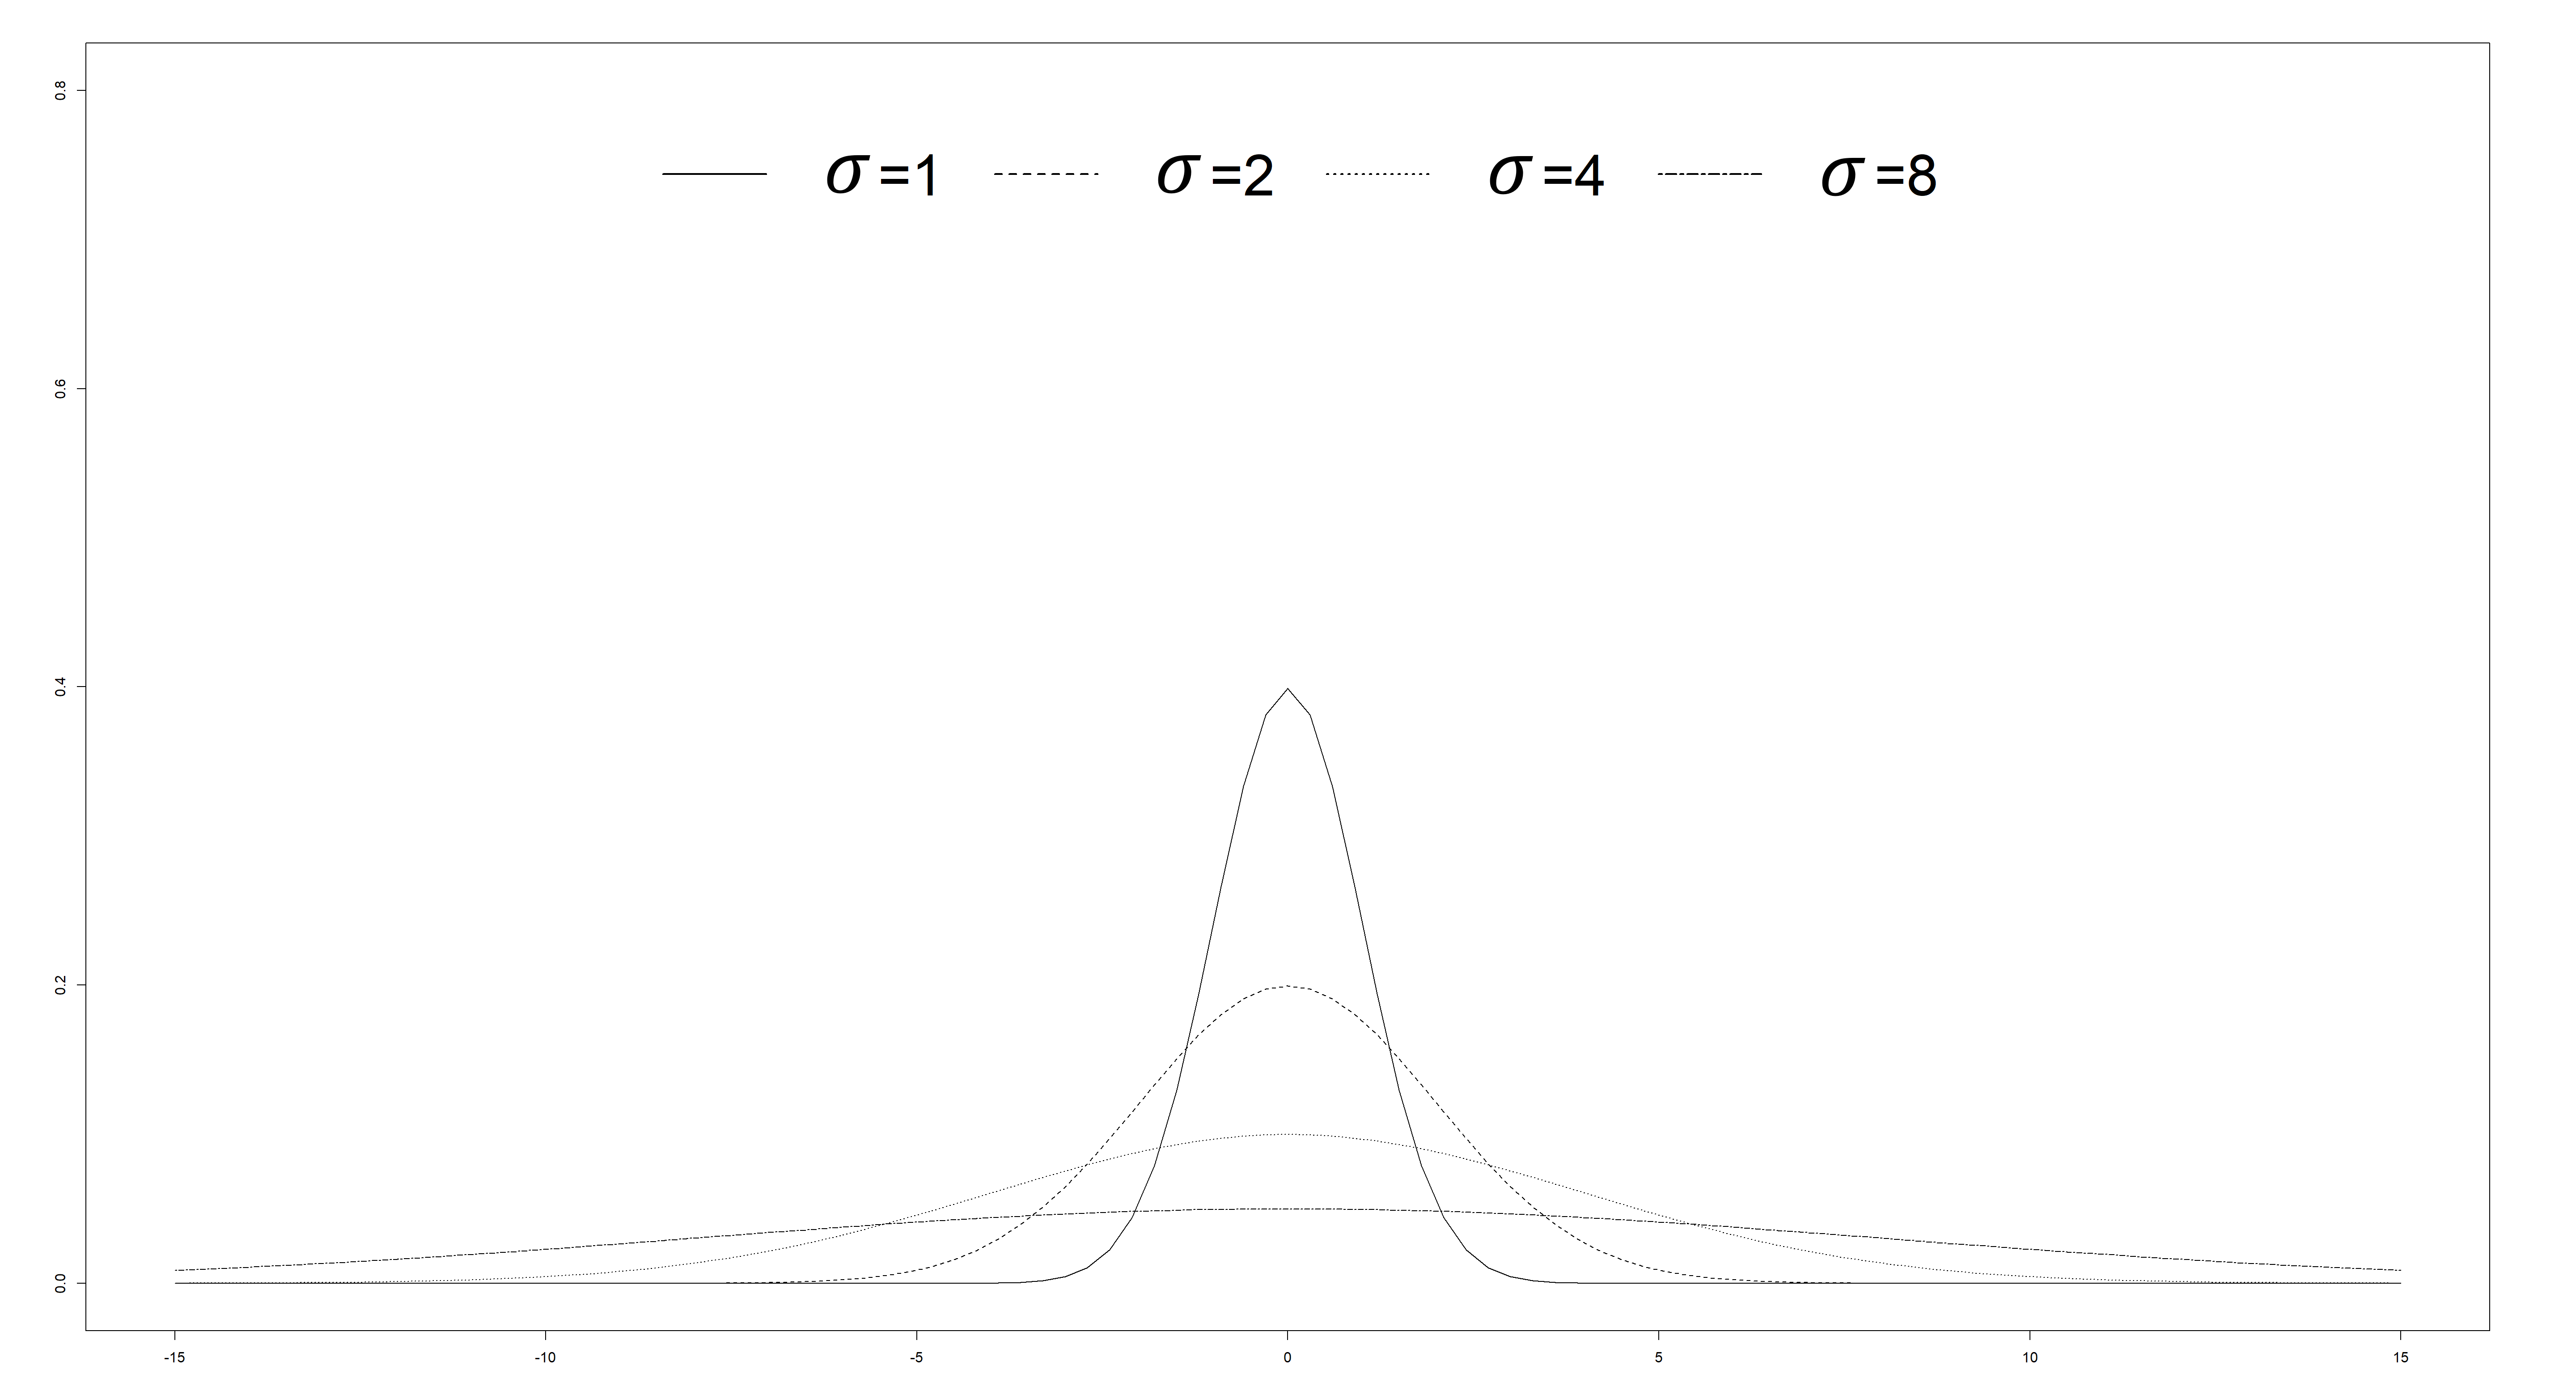
\includegraphics{C:/Users/mdelacre/Documents/Github project/thesis/Chapitre 3/Appendix figures/1_normal.png}
\caption{``Figure A1 : centered normal probability density function, as
a function of the population SD''}
\end{figure}

\begin{figure}
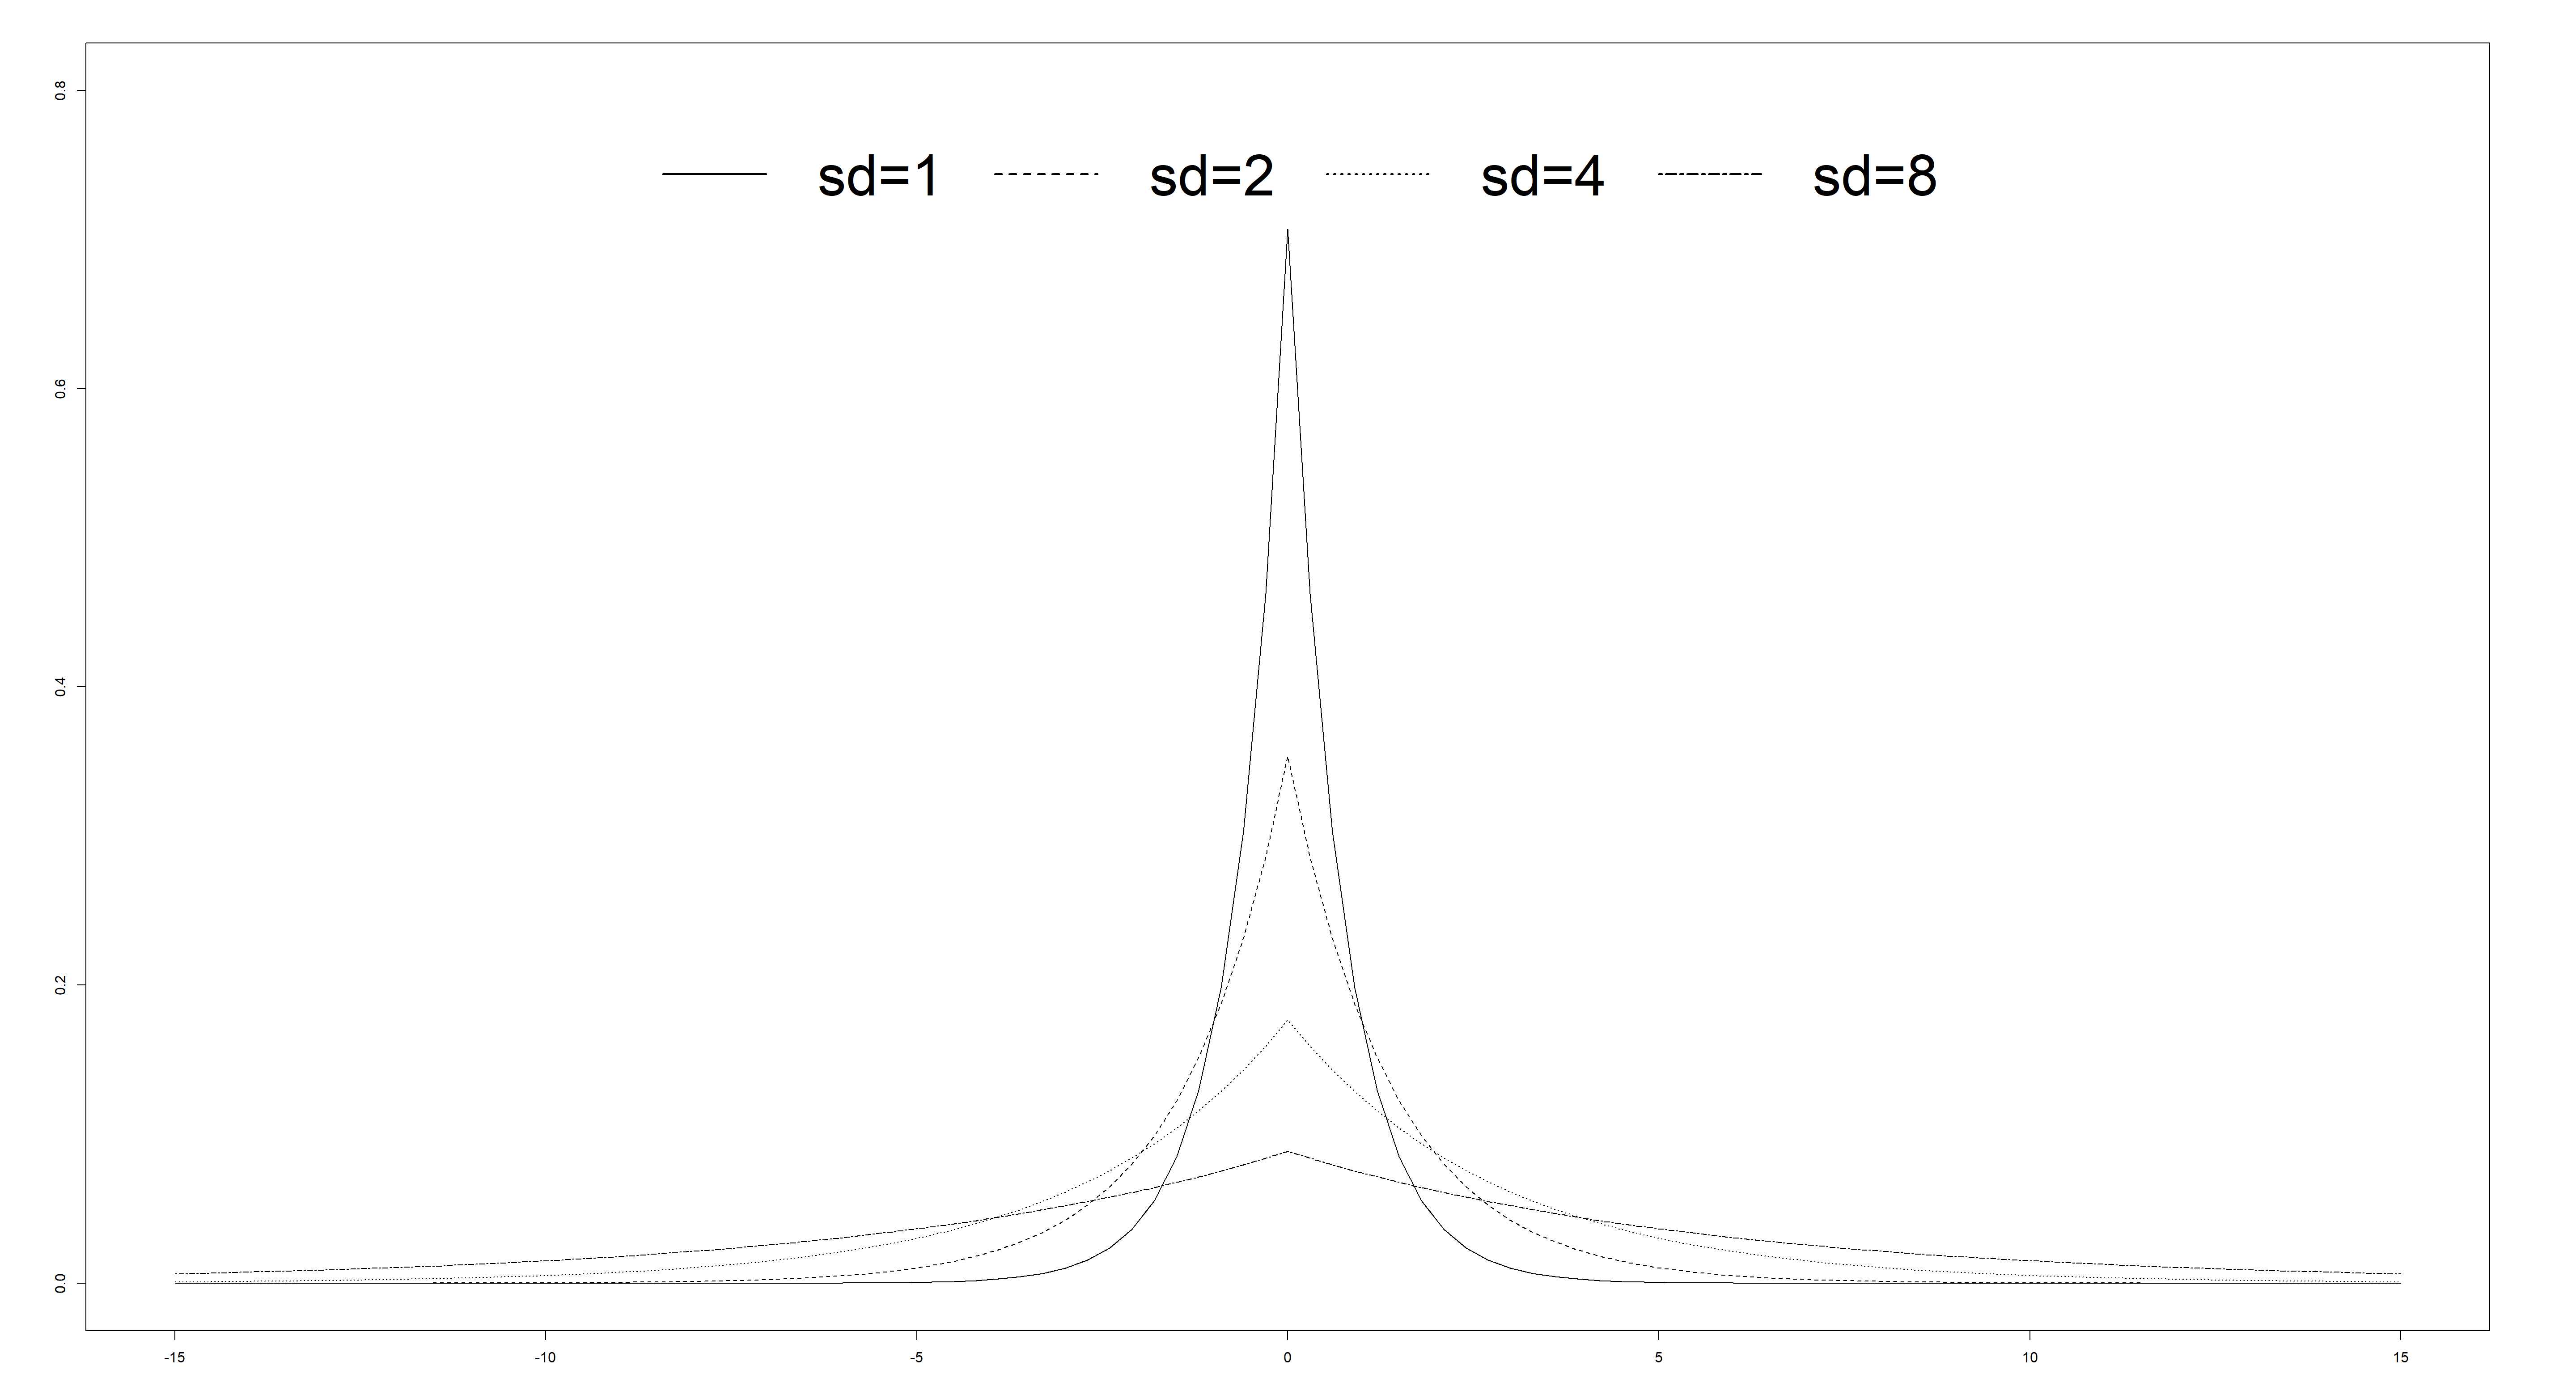
\includegraphics[width=400px]{C:/Users/mdelacre/Documents/Github project/thesis/Chapitre 3/Appendix figures/2_doublex} \caption{centered double exponential probability density function, as a function of the population SD}\label{fig:unnamed-chunk-4}
\end{figure}

\begin{figure}
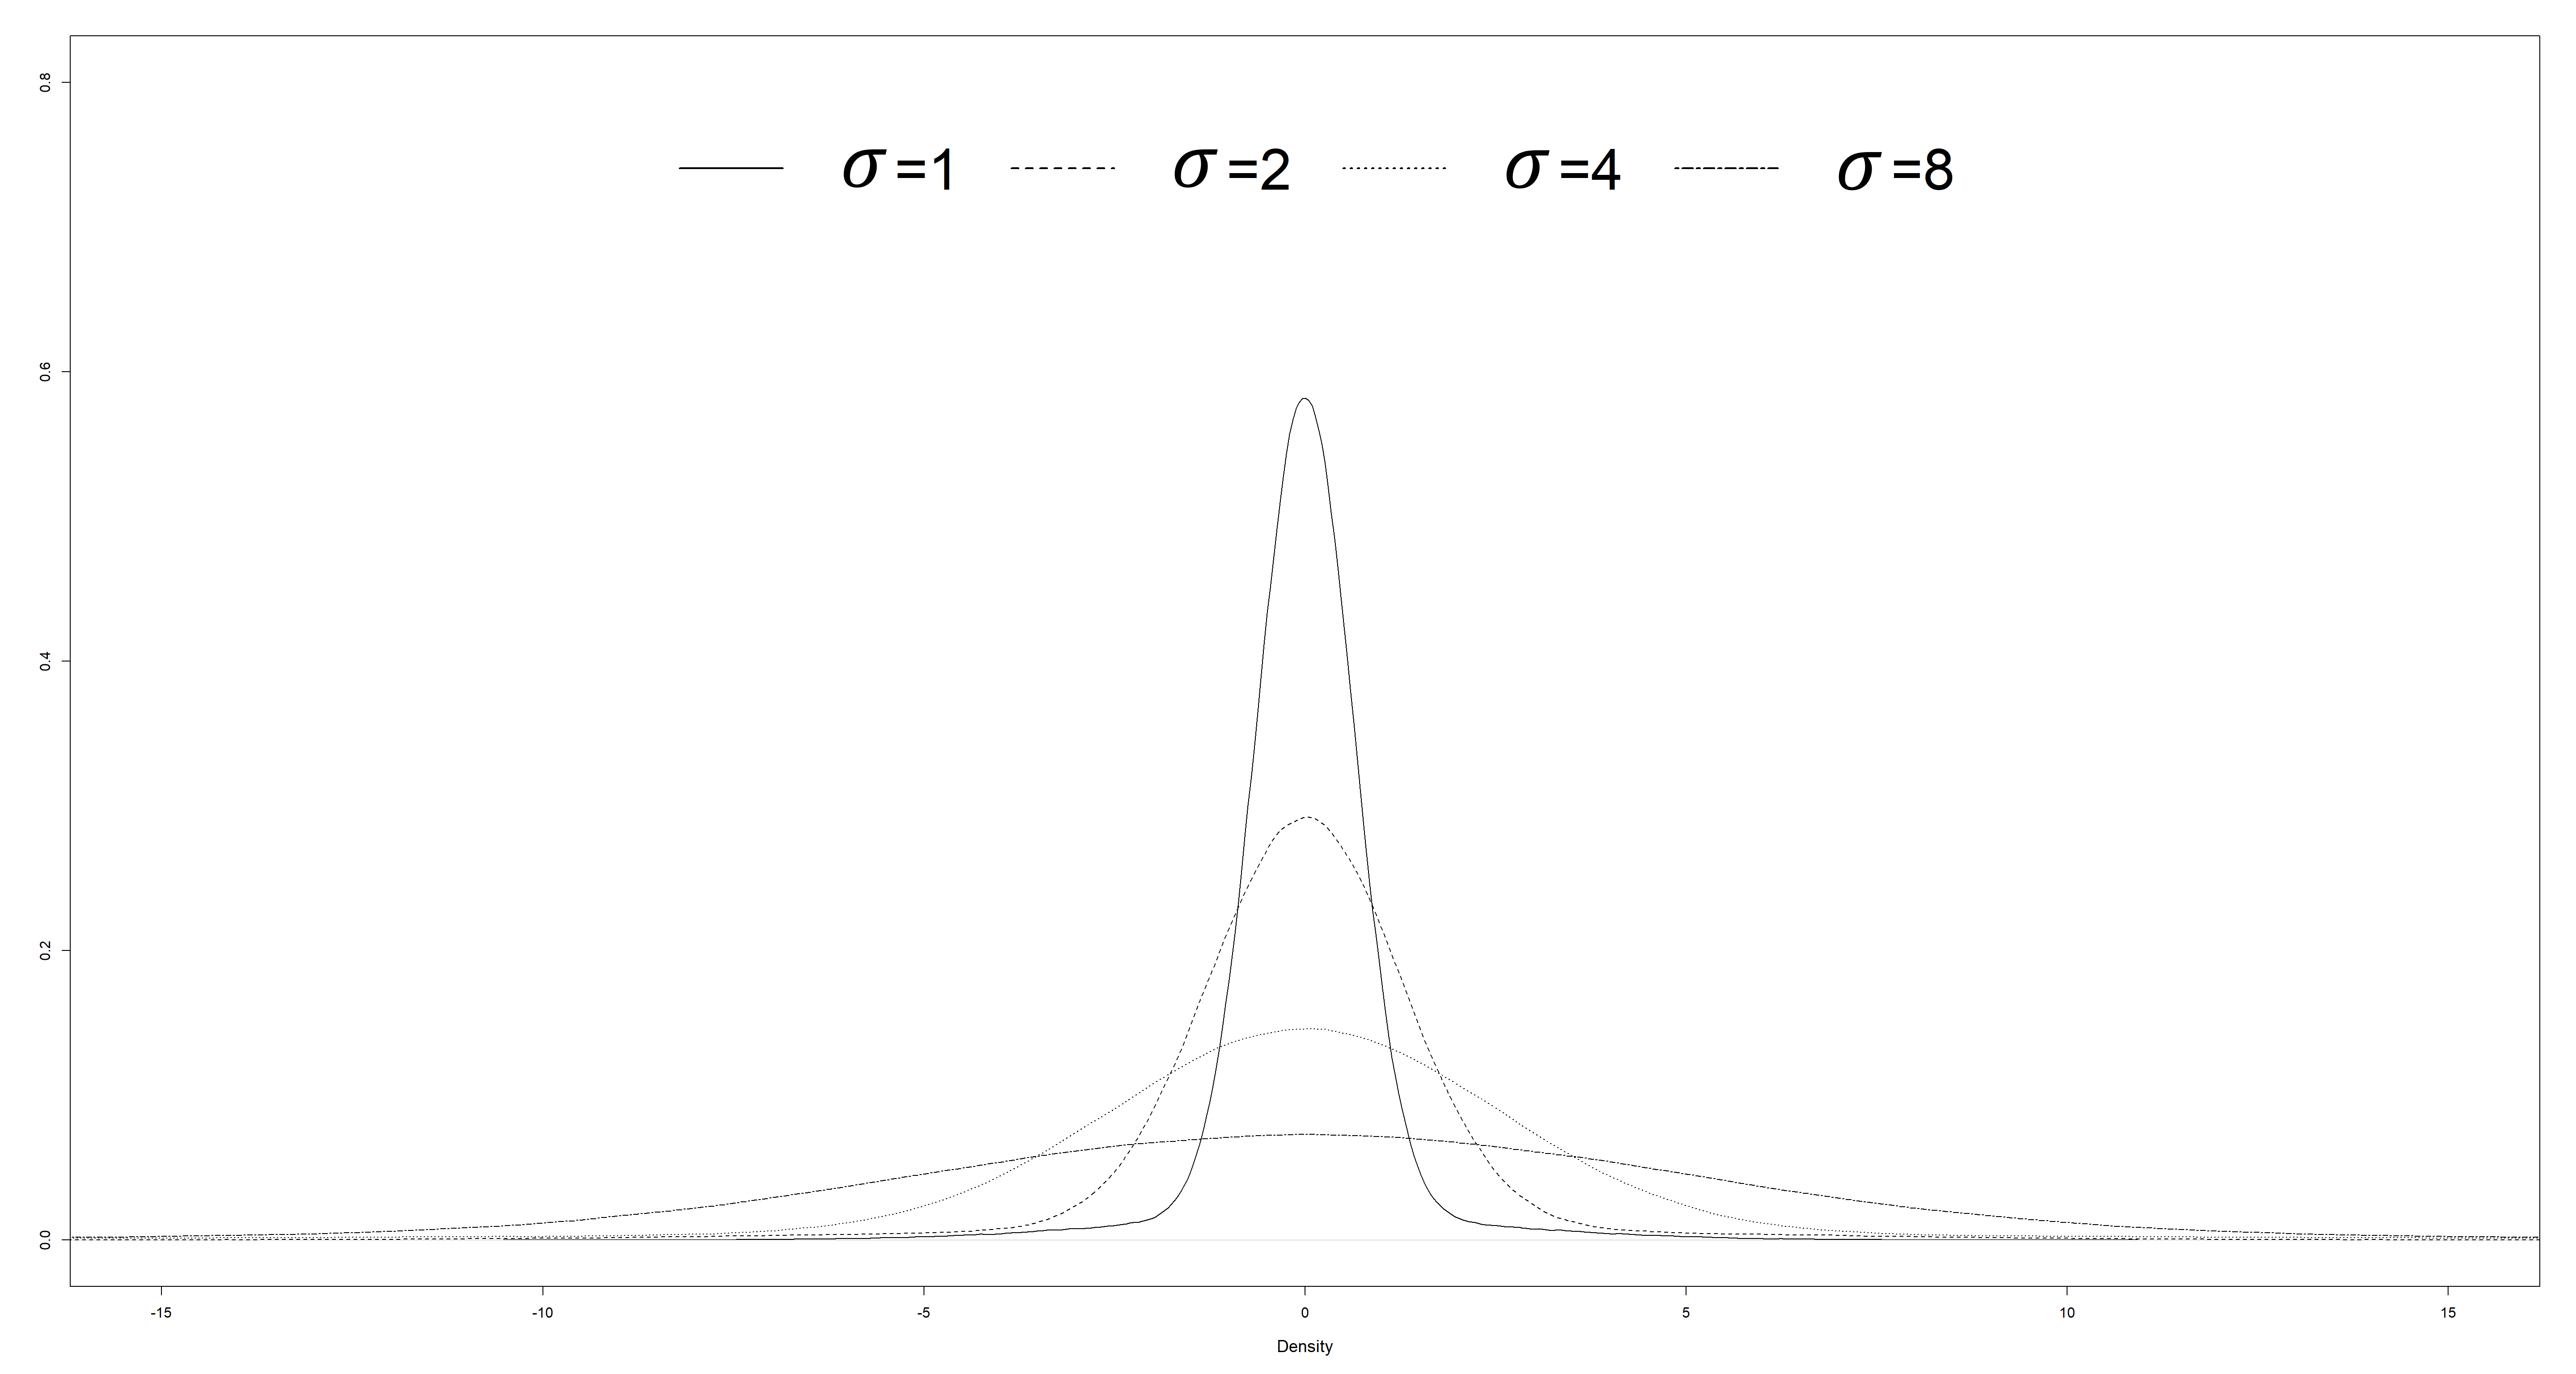
\includegraphics[width=400px]{C:/Users/mdelacre/Documents/Github project/thesis/Chapitre 3/Appendix figures/3_mixednorm} \caption{centered mixed normal probability density function, as a function of the population SD}\label{fig:unnamed-chunk-5}
\end{figure}

\begin{figure}
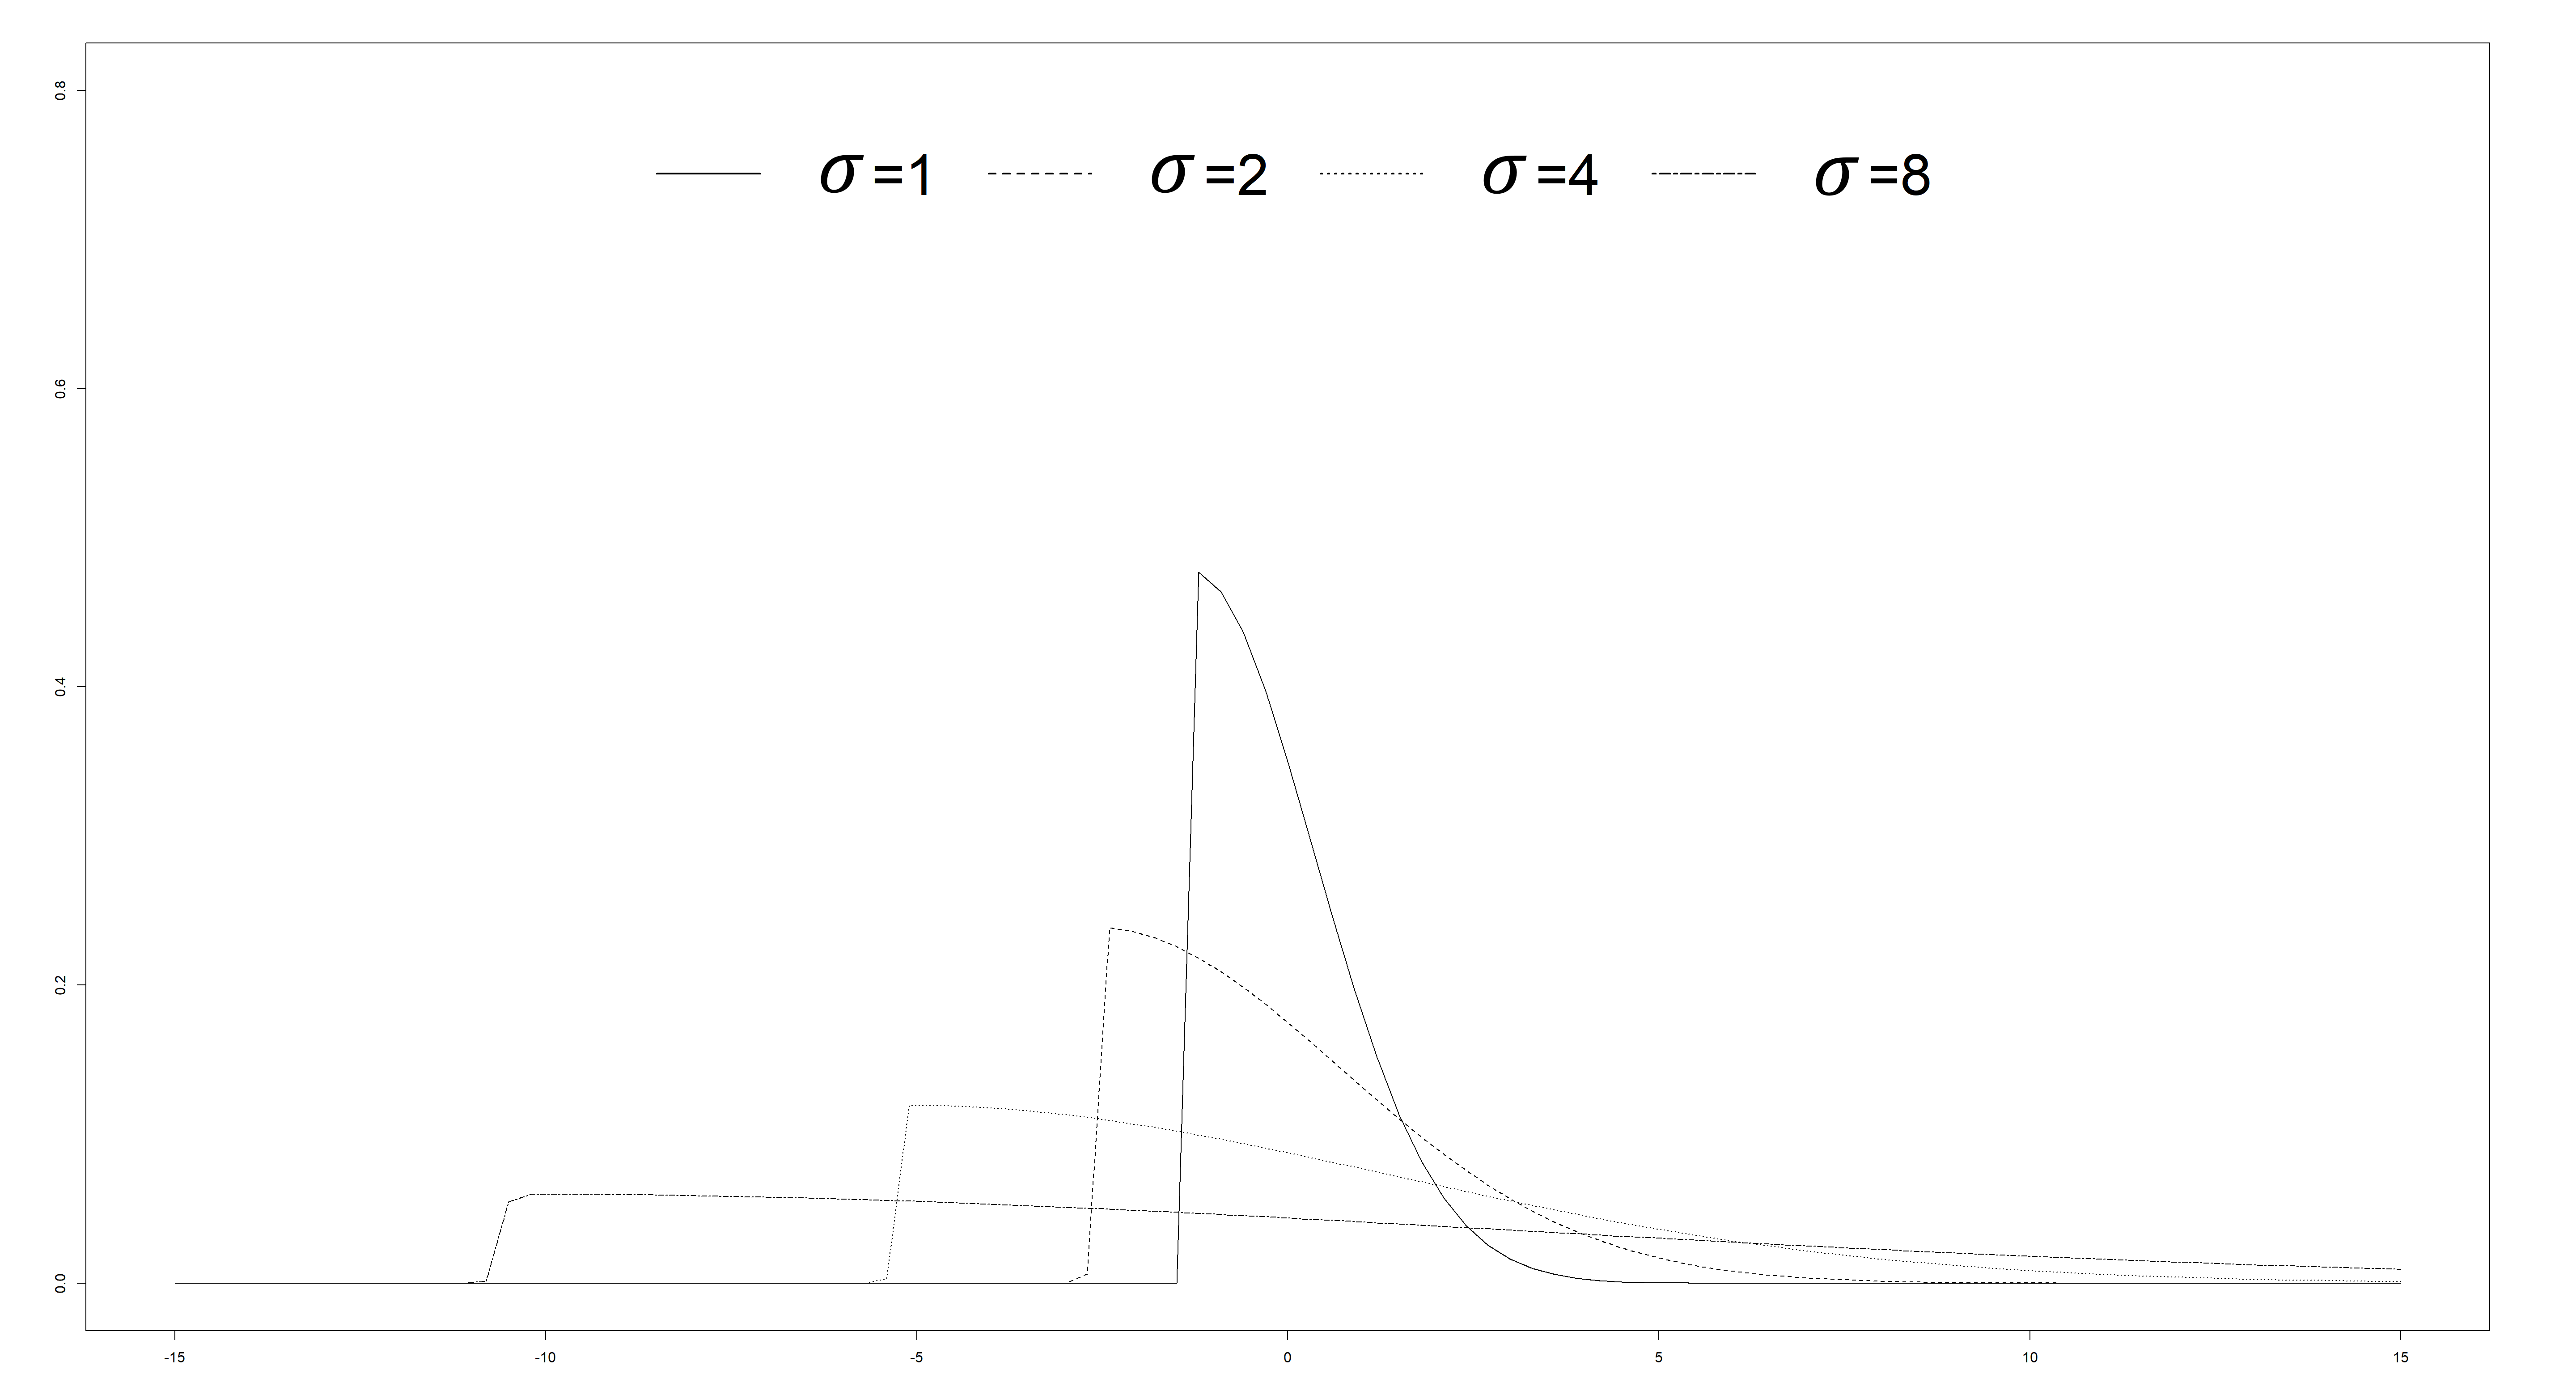
\includegraphics[width=400px]{C:/Users/mdelacre/Documents/Github project/thesis/Chapitre 3/Appendix figures/4_rightskewed} \caption{centered normal right skewed probability density function, as a function of the population SD}\label{fig:unnamed-chunk-6}
\end{figure}

\begin{figure}
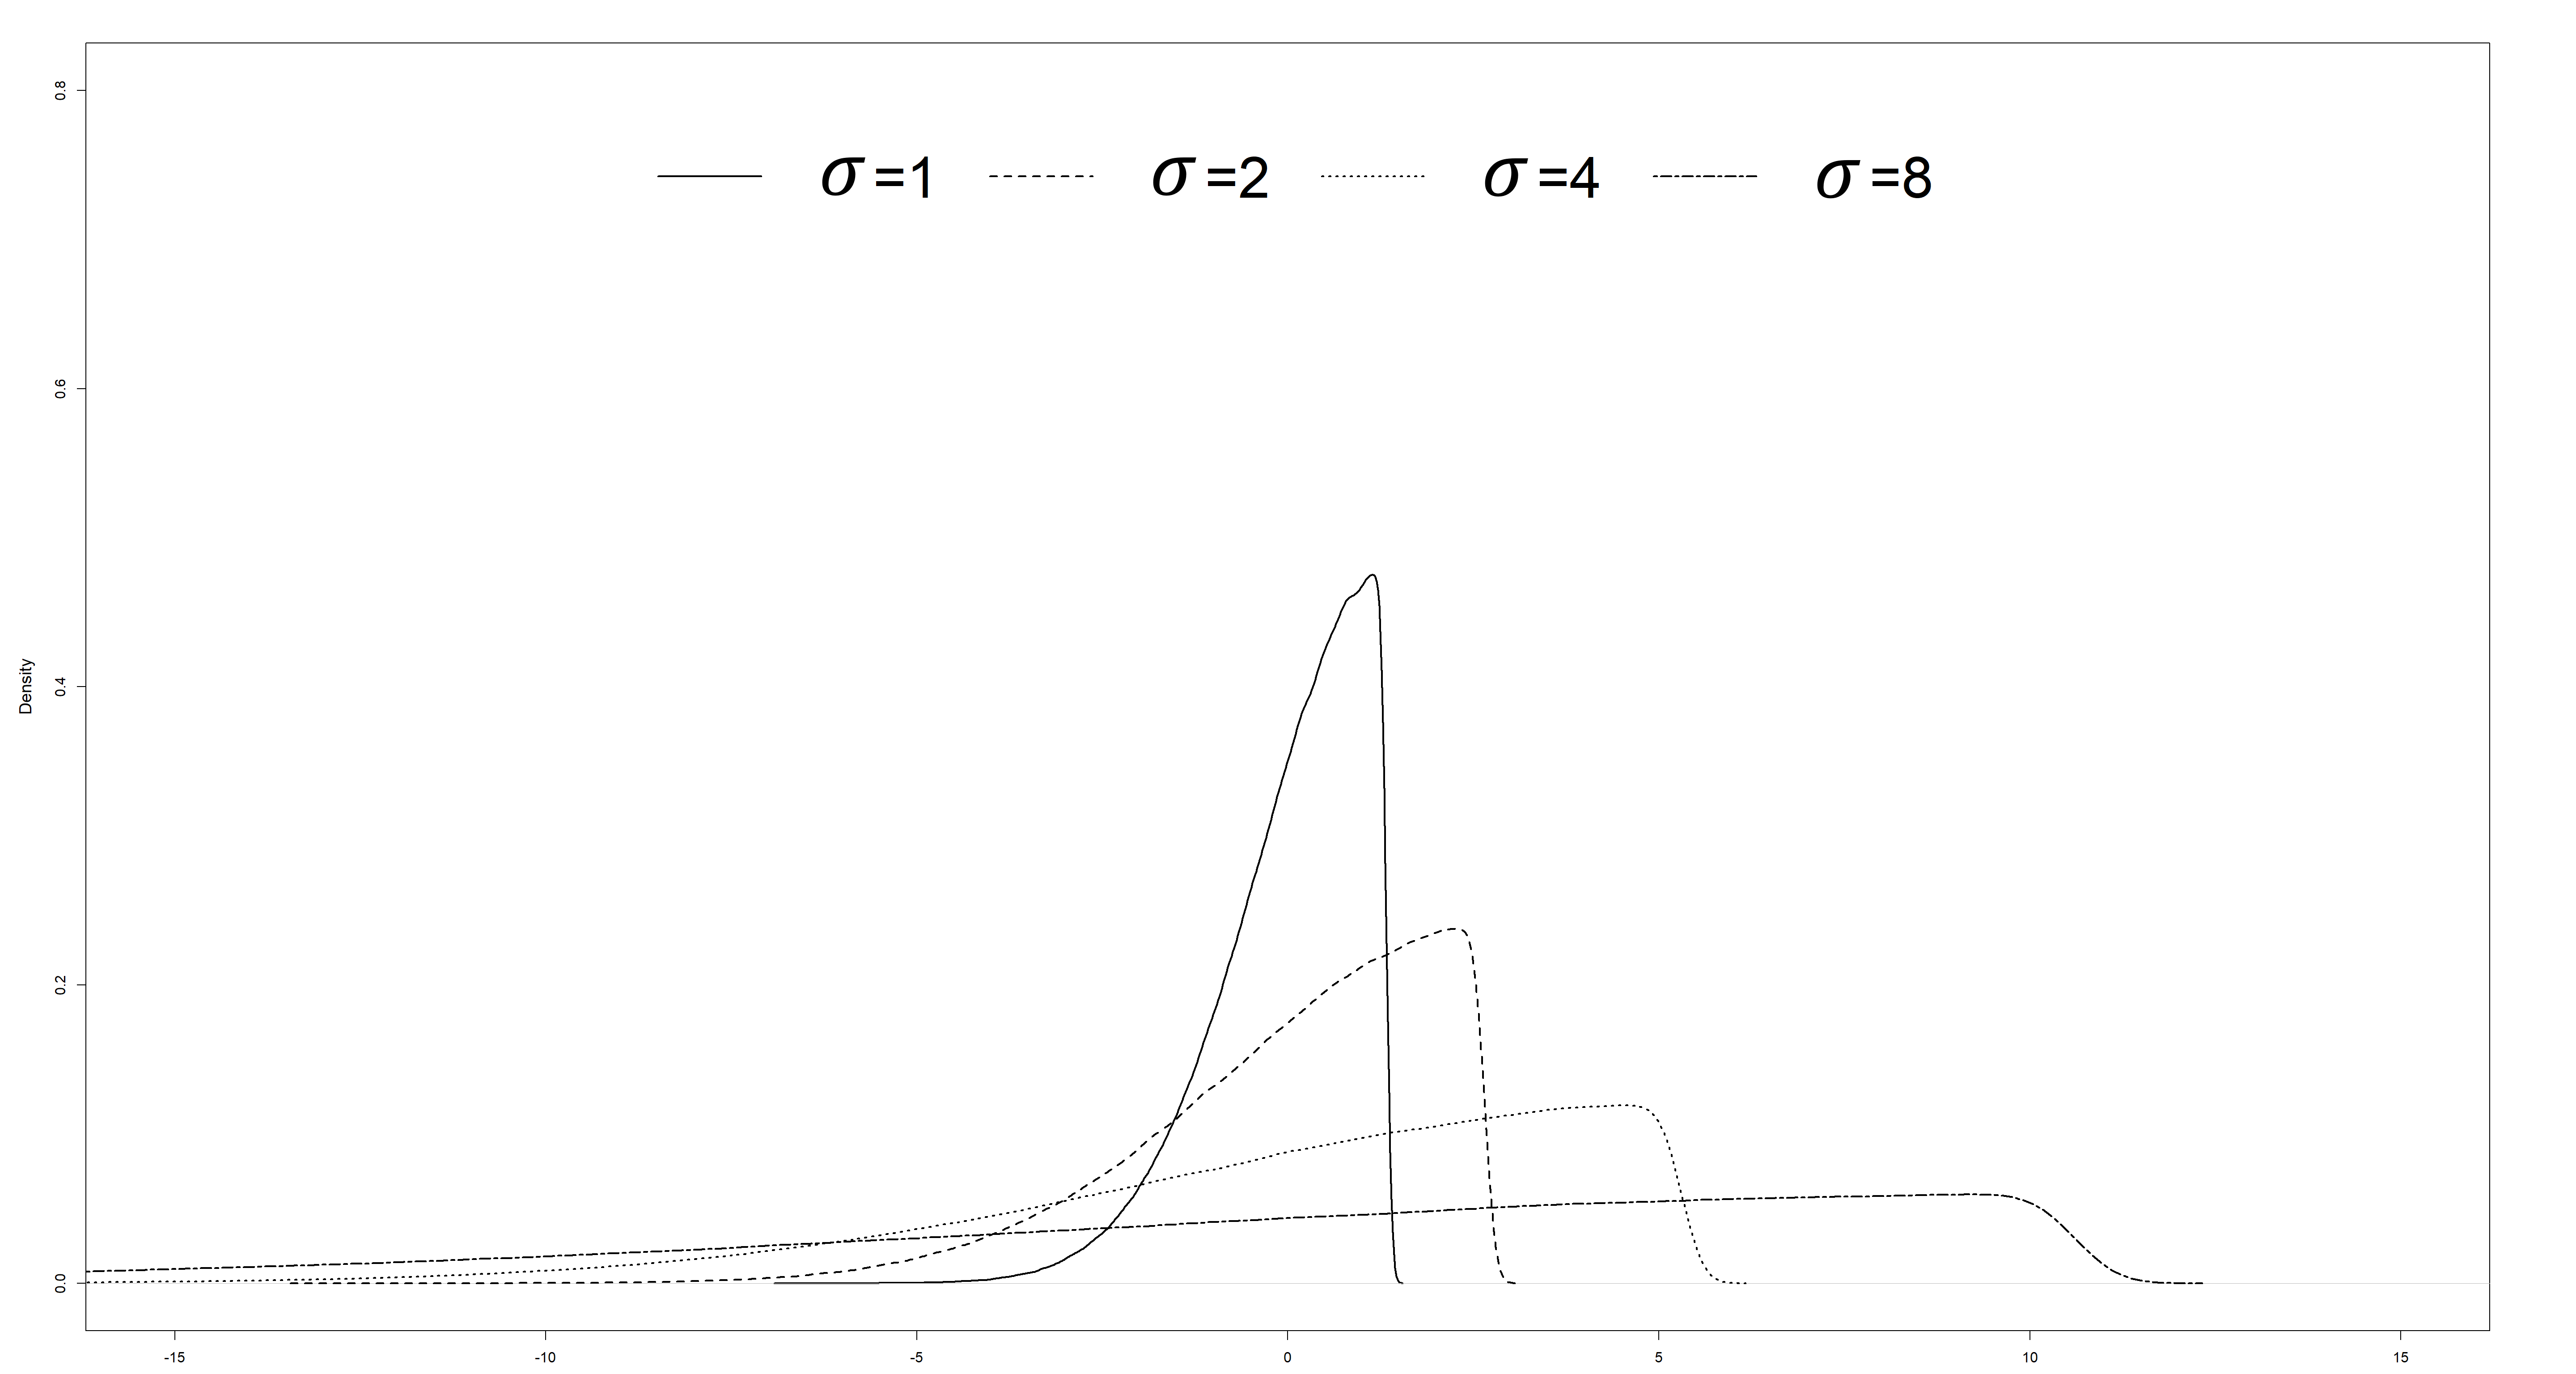
\includegraphics[width=400px]{C:/Users/mdelacre/Documents/Github project/thesis/Chapitre 3/Appendix figures/5_leftskewed} \caption{centered normal left skewed probability density function, as a function of the population SD}\label{fig:unnamed-chunk-7}
\end{figure}

\begin{figure}
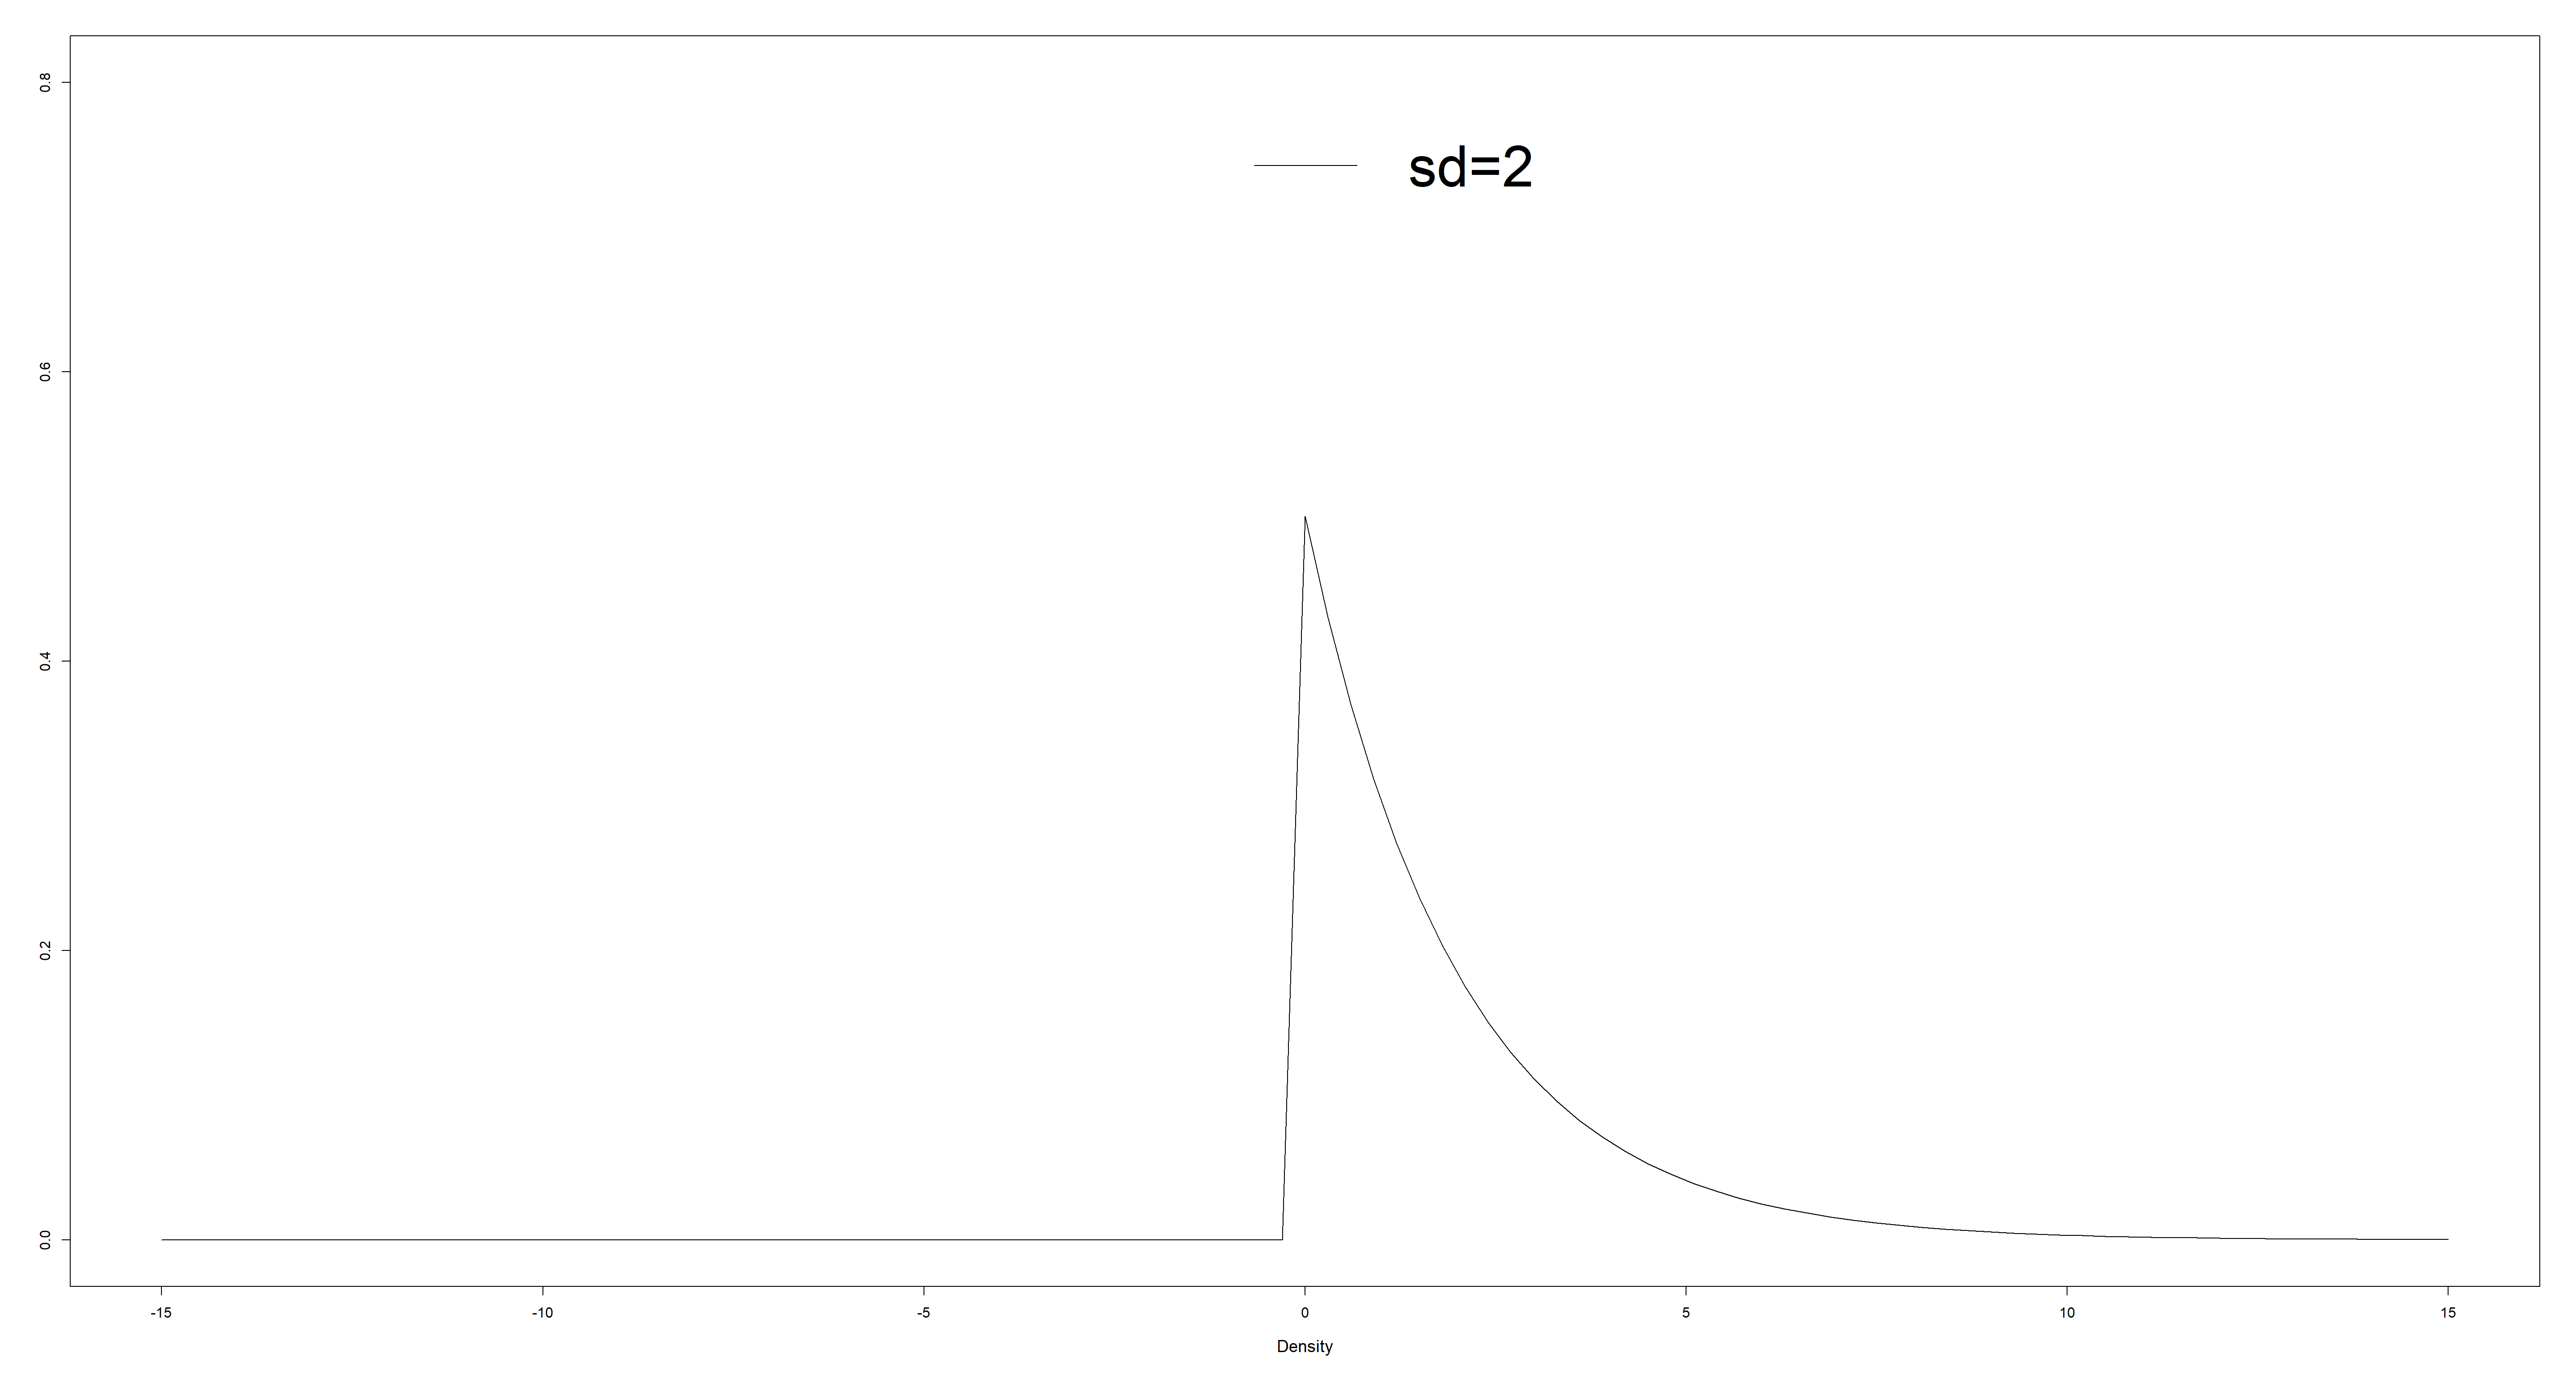
\includegraphics[width=400px]{C:/Users/mdelacre/Documents/Github project/thesis/Chapitre 3/Appendix figures/6_chisquared} \caption{chi-squared with 2 degrees of freedom probability density function, when SD=2}\label{fig:unnamed-chunk-8}
\end{figure}

\newpage

\hypertarget{annexes-du-chapitre-4}{%
\subsection{Annexes du Chapitre 4}\label{annexes-du-chapitre-4}}

\hypertarget{appendix-1-the-bias-of-cohens-bmd-is-twice-as-large-as-the-bias-of-shiehs-bmd-when-population-variances-and-sample-sizes-are-equal-across-groups-mathematical-demonstration.}{%
\subsubsection{\texorpdfstring{Appendix 1 : The bias of Cohen's
\(\bm{d}\) is twice as large as the bias of Shieh's \(\bm{d}\) when
population variances and sample sizes are equal across groups:
mathematical
demonstration.}{Appendix 1 : The bias of Cohen's \textbackslash bm\{d\} is twice as large as the bias of Shieh's \textbackslash bm\{d\} when population variances and sample sizes are equal across groups: mathematical demonstration.}}\label{appendix-1-the-bias-of-cohens-bmd-is-twice-as-large-as-the-bias-of-shiehs-bmd-when-population-variances-and-sample-sizes-are-equal-across-groups-mathematical-demonstration.}}

As mentioned in Table 2, the bias of Cohen's \(d\) is defined as
\begin{equation} 
Bias_{Cohen's \; d}= \delta_{Cohen} \times \left( \frac{\sqrt{\frac{df_{Student}}{2}} \times \Gamma{\left(\frac{df_{Student}-1}{2}\right)}}{\Gamma{\left( \frac{df_{Student}}{2}\right)}} -1 \right)
(\#eq:Cohenbias)
\end{equation} with \begin{equation*} 
\delta_{Cohen}=\frac{\mu_1-\mu_2}{\sqrt{\frac{(n_1-1)\times \sigma^2_1+(n_2-1)\times\sigma^2_2}{n_1+n_2-2}}}
(\#eq:Cohendelta)
\end{equation*} and \begin{equation*} 
df_{Student}=n_1+n_2-2
(\#eq:Cohendf)
\end{equation*}

As mentioned in Table 3, the bias of Shieh's \(d\) is defined as
\begin{equation} 
Bias_{Shieh's \; d}=\delta_{Shieh} \times \left( \frac{\sqrt{\frac{df_{Welch}}{2}} \times \Gamma{\left(\frac{df_{Welch}-1}{2}\right)}}{\Gamma{\left( \frac{df_{Welch}}{2}\right)}} -1 \right)
(\#eq:Shiehbias)
\end{equation} with \begin{equation*} 
\delta_{Shieh}=\frac{\mu_1-\mu_2}{\sqrt{\frac{\sigma^2_1}{n_1/N}+\frac{\sigma^2_2}{n_2/N}}} \quad (N=n_1+n_2)
(\#eq:Shiehdelta)
\end{equation*} and \begin{equation*} 
df_{Welch}=\frac{\left(\frac{\sigma^2_1}{n_1}+\frac{\sigma^2_2}{n_2} \right)^2}{\frac{(\sigma^2_1/n_1)^2}{n_1-1}+\frac{(\sigma^2_2/n_2)^2}{n_2-1}}
(\#eq:Welchdf)
\end{equation*}

When \(n_1=n_2=n\) and \(\sigma_1=\sigma_2=\sigma\), \(\delta_{Cohen}\)
is twice larger than \(\delta_{Shieh}\), as shown below in equations
\ref{eq:Cohendeltavarbalanced} and \ref{eq:Shiehdeltavarbalanced}:
\begin{equation} 
\delta_{Cohen}=\frac{\mu_1-\mu_2}{\sqrt{\frac{2(n-1)\sigma^2}{2(n-1)}}}=\bm{\frac{\mu_1-\mu_2}{\sigma}}
(\#eq:Cohendeltavarbalanced)
\end{equation} \begin{equation} 
\delta_{Shieh}=\frac{\mu_1-\mu_2}{\sqrt{2\left( \frac{\sigma^2}{n/(2n)}\right)}}=\bm{\frac{\mu_1-\mu_2}{2\sigma}} 
(\#eq:Shiehdeltavarbalanced)
\end{equation}\\
Moreover, degrees of freedom associated with Student's \emph{t}-test and
Welch's \emph{t}-test are identical, as shown below in equations
\ref{eq:Studentdfvarbalanced} and \ref{eq:Welchdfvarbalanced}:
\begin{equation} 
df_{Student}=\bm{2(n-1)} 
(\#eq:Studentdfvarbalanced)
\end{equation} \begin{equation} 
df_{Welch}=\frac{\left[2(\sigma^2/n)\right]^2}{\frac{2(\sigma^2/n)^2}{n-1}}= \bm{2(n-1)} 
(\#eq:Welchdfvarbalanced)
\end{equation}

Equations \ref{eq:Cohenbias} and \ref{eq:Shiehbias} can therefore be
redefined as follows: \begin{equation} 
Bias_{Cohen's \; d}=\frac{\mu_1-\mu_2}{\sigma} \times \left( \frac{\sqrt{n-1} \times \Gamma{\left(\frac{2n-3}{2}\right)}}{\Gamma{\left( n-1\right)}} -1 \right)
(\#eq:Cohenbiasvarbalanced)
\end{equation} \begin{equation} 
Bias_{Shieh's \; d}=\frac{\mu_1-\mu_2}{\bf 2\sigma} \times \left( \frac{\sqrt{n-1} \times \Gamma{\left(\frac{2n-3}{2}\right)}}{\Gamma{\left( n-1\right)}} -1 \right)
(\#eq:Shiehbiasvarbalanced)
\end{equation}

We can therefore conclude that the bias of Cohen's \(d\) is twice larger
than the bias of Shieh's \(d\).

\newpage

\hypertarget{appendix-2-the-variance-of-cohens-bmd-is-four-times-larger-than-the-bias-of-shiehs-bmd-when-population-variances-and-sample-sizes-are-equal-across-groups-mathematical-demonstration.}{%
\subsubsection{\texorpdfstring{Appendix 2 : The variance of Cohen's
\(\bm{d}\) is four times larger than the bias of Shieh's \(\bm{d}\) when
population variances and sample sizes are equal across groups:
mathematical
demonstration.}{Appendix 2 : The variance of Cohen's \textbackslash bm\{d\} is four times larger than the bias of Shieh's \textbackslash bm\{d\} when population variances and sample sizes are equal across groups: mathematical demonstration.}}\label{appendix-2-the-variance-of-cohens-bmd-is-four-times-larger-than-the-bias-of-shiehs-bmd-when-population-variances-and-sample-sizes-are-equal-across-groups-mathematical-demonstration.}}

The variance of Cohen's \(d\) is defined in Table 2 as \begin{equation}
Var_{Cohen's \; d}=\frac{N\times df_{Student}}{n_1n_2 \times (df_{Student}-2)} + \delta^2_{Cohen} \left[ \frac{df_{Student}}{df_{Student}-2} - \left( \frac{\sqrt{\frac{df_{Student}}{2}} \times \Gamma{\left(\frac{df_{Student}-1}{2}\right)}}{\Gamma{\left( \frac{df_{Student}}{2}\right)}} \right)^2\right]
(\#eq:Cohenvar)
\end{equation} and the variance of Shieh's \(d\) is defined in Table 2
as \begin{equation}
Var_{Shieh's \; d}=\frac{df_{Welch}}{(df_{Welch}-2)N}  + \delta^2_{Shieh} \left[ \frac{df_{Welch}}{df_{Welch}-2} - \left( \frac{\sqrt{\frac{df_{Welch}}{2}} \times \Gamma{\left(\frac{df_{Welch}-1}{2}\right)}}{\Gamma{\left( \frac{df_{Welch}}{2}\right)}} \right)^2 \right]
(\#eq:Shiehvar)
\end{equation}

We have previously shown in equations \ref{eq:Studentdfvarbalanced} and
\ref{eq:Welchdfvarbalanced} that degrees of freedom associated with
Student's \emph{t}-test and Welch's \emph{t}-test equal \(2(n-1)\), when
\(n_1=n_2=n\) and \(\sigma_1=\sigma_2=\sigma\). As a consequence, the
first term of the addition in equation \ref{eq:Cohenvar} is 4 times
larger than the first term of the addition in equation
\ref{eq:Shiehvar}:
\[\frac{N\times df_{Student}}{n_1n_2 \times (df_{Student}-2)}=\frac{2n\times 2(n-1)}{n^2 \times (2n-4)} =\bm{\frac{4(n-1)}{n(2n-4)}} \]
\[\frac{df_{Welch}}{(df_{Welch}-2)N} = \frac{2(n-1)}{2n(2n-4)}= \bm{\frac{n-1}{n(2n-4)}}\]
We have also previously shown in equations
\ref{eq:Cohendeltavarbalanced} and \ref{eq:Shiehdeltavarbalanced} that
\(\delta_{Cohen}\) is twice larger than \(\delta_{Shieh}\) when
\(n_1=n_2=n\) and \(\sigma_1=\sigma_2=\sigma\) and, therefore,
\(\delta^2_{Cohen}\) is four times larger than \(\delta^2_{Shieh}\). As
a consequence, the second term of the addition in equation
\ref{eq:Cohenvar} is also 4 times larger than the second term of the
addition in equation \ref{eq:Shiehvar}. Because both terms of the
addition in equation \ref{eq:Cohenvar} are four times larger than those
in equation \ref{eq:Shiehvar}, we can conclude that the variance of
Cohen's \(d\) is four times larger than the variance of Shieh's \(d\).

\end{document}
